\chapter{Coupled Cluster Theory}
\label{ch:coupled}

Coupled cluster theory was developed by Fritz Coester and Hermann 
K\"ummel, \cite{Coester1958421} and \cite{Coester1960477}. It is a method used to describe many-body systems. 
The method starts with a ground state Slater determinant, as the Slater determinant below, Eq.\eqref{slaterdet}, which corresponds to a system consisting of four particles
\be
\Phi_0=\frac{1}{\sqrt{4!}}
\left|
\begin{array}{cccc}
\phi_i(x_1) & \phi_j(x_1) & \phi_k(x_1) & \phi_l(x_1)\\
\phi_i(x_2) & \phi_j(x_2) & \phi_k(x_2) & \phi_l(x_2)\\
\phi_i(x_3) & \phi_j(x_3) & \phi_k(x_3) & \phi_l(x_3)\\
\phi_i(x_4) & \phi_j(x_4) & \phi_k(x_4) & \phi_l(x_4)\\
\end{array}
\right|.
\label{slaterdet}
\ee
A convenient shorthand notation for the Slater determinant consists of a 
Dirac-notation ket containing only the diagonal elements of the Slater 
determinant, see Ref. \cite{sjefer}.
The ket vector corresponding to Eq.~\eqref{slaterdet} would 
be written as
\be
\ket{\phi_i( x_1)\phi_j(x_2)\phi_k( x_3) \phi_l( x_4)}.
\ee
This independent particle model does not consider the effects from the interactions beyond the uncorrelated wavefunction $\Phi_0$ we get by filling the $N$ single-particle orbitals with lowest energy. To include the effects beyond the uncorrelated wavefunction we make an ansatz and write the coupled cluster wavefunction
as
\be
\Psi=e^T \Phi_0,
\ee
where $T$ is a cluster operator, not to be confused with the kinetic energy and $\ket{\Phi_0}$ is our reference vacuum. The cluster operator $T$ is a linear combination of different types of excitations and written as
\be
T=T_1+T_2+T_3 + \cdots
\ee
The symbol $T_1$ is an operator of all single excitations, and $T_2$ the operator of 
all double excitations, and so on. 
By the formalism of the second quantization the excitation operators are expressed as 
\begin{align}
& T_1 = \sum_{ia} t^a_ia^\dagger_a a_i 
\end{align}
and
\begin{align}
& T_2 = \frac{1}{4} \sum_{ijab} t^{ab}_{ij} a^\dagger_aa^\dagger_ba_ja_i. 
\end{align}
More generally an $n-$orbital cluster operator may be defined as %Ref. \cite{sjefer} 
\be
T_n = \left(\frac{1}{n!}\right)^2 \sum_{ij \dots ab \dots} t^{ab\dots}_{ij 
\dots} a^\dagger_aa^\dagger_b \dots a_ja_i. 
\ee
The new correlated wavefunction is a linear expansion of several Slater determinants which are considered as
excitations of $\ket{\Phi_0}$.
The cluster amplitudes, $t^a_i,t^{ab}_{ij}$ etc., are to be determined via
the Schr\"odinger equation, see for instance Ref.~\cite{sjefer}.\\
The new wavefunction $\ket{\Psi}$ satisfies the Schr\"odinger equation as 
written below
\begin{equation*}
		H\ket{\Psi}=He^T\ket{\Phi_0}=Ee^T\ket{\Phi_0}=E\ket{\Psi}.
		\label{nyepsi}
\end{equation*}
To obtain an expression for the energy, the reference wave-function $\Phi_0$ is multiplied from left with the Schr\"odinger. We obtain
\begin{equation*}
		\bra{\Phi_0}He^T\ket{\Phi_0}.
\end{equation*}
However it has turned out to be convenient to multiply the Schr\"odinger equation, Eq.~\eqref{nyepsi} with $e^{-T}$ and then do a left-projection by the reference $\Phi_0$, to get
\be
E = \bra{\Phi_0}e^{-T}He^T \ket{\Phi_0}. 
\label{coupleenergy}
\ee
By using the Campbell-Baker-Hausdorff formula on $e^{-T}He^T$, Eq. \eqref{coupleenergy} transforms to
\beq
E = \bra{\Phi_0} H +[H,T_1] + [H,T_2] + \frac{1}{2}[[H,T_1],T_1]+ \frac{1}{2}[[H,T_2],T_2] + [[H,T_1],T_2] + \cdots \ket{\Phi_0}.
\eeq 
We have here truncated the cluster operator at $T_2$. The above expression is valid even at higher truncations as long as the Hamiltonian just consists of a two body operator.\\
Different truncations are denoted by short-hand notations, for instance a truncation on $T_1$ is called a CCS approach, a truncation on $T_2$  a CCSD approach and a truncation on $T_2$ without considering the $T_1$ amplitudes is called a CCD approach.\\
%Ref. \cite{MortenogD.J.Dean}% Toward coupled cluster implementations in Nucl strct
\\
In order to find the energy of the system we need to determine the amplitudes $t_i^a$ and $t^{ab}_{ij}$. This is done by using the orthogonality properties
\begin{equation}
%\begin{split}
 \bra{\Phi^a_i}e^{-T}He^T\ket{\Phi_0}=0,
\label{cclikn1}
\end{equation}
and
\begin{equation}
 \bra{\Phi^{ab}_{ij}}e^{-T}He^T\ket{\Phi_0}=0.
%\end{split}
\label{cclikn2}
\end{equation}
The above equations are to be derived in the following sections. Since we in this work have truncated the cluster operator at $T_2$, the equations
\eqref{cclikn1} and \eqref{cclikn2} are the 
only equations needed in order to determine the cluster amplitudes $t^a_i$ and $t^{ab}_{ij}$.

\section{The CCSD energy equation}

The energy problem simplifies when the normalized Hamiltonian, $H_N$, 
according to the quasiparticle formalism, is used, see Eq.~\eqref{normalham}. In the last section an 
expansion on $e^{-T}He^T$ was derived by the Campbell-Baker-Hausdorff formula. 
When our Hamiltonian is at most a two particle operator, this expression will be
truncated at
\be
\begin{split}
& e^{-T} H_Ne^T =H_N +[H_N,T_1] + [H_N,T_2] + \\& \frac{1}{2}[[H_N,T_1],T_1]+ \frac{1}{2}[[H_N,T_2],T_2] + [[H_N,T_1],T_2],
\label{hausd}
\end{split}
\ee
where 
\be
H_N=\sum_{\alpha\beta}f_{\alpha\beta}N(a^\dagger_\alpha a_\beta)+
\frac{1}{4}\sum_{\alpha\beta\gamma\delta}v_{\alpha\beta\gamma\delta}N(
a^\dagger_\alpha a^\dagger_\beta a_\delta a_\gamma)
\label{normha}
\ee
is the normal ordered Hamiltonian as in chapter \ref{chapsecondq}, with 
\beq
f_{\alpha\beta}=\bra{\alpha}h\ket{\beta}+ \frac{1}{4}\sum_i \bra{\alpha i}v\ket{i\beta}~\mbox{and}~v_{\alpha\beta\gamma\delta}=\bra{\alpha\beta}v\ket{\gamma\delta}.
\eeq
The first order correction to the energy,
\beq
E_0=\sum_i \bra{i}h\ket{i}+\frac{1}{2}\sum_{ij}\bra{ij}v\ket{ij},
\eeq
see Eq.\eqref{normalham}, is left out.
%When the expectation value of this expression is computed, only three terms
%will survive.
%Since the expression for the normalized Hamiltonian is already calculated in
%Eq. \eqref{normalham} and given again in Eq. \eqref{normha}.
By taking the expectation value of the expanded normal ordered Hamiltonian, 
Eq.~\eqref{hausd}, with the reference vacuum, $\Phi_0$,
we see that the first term, $H_N$ of the expansion in Eq.~\eqref{hausd} falls out. However the $H_N$ term will contribute in the amplitude equations.\\
\\
We will now go thoroughly through the terms in Eq.~\eqref{hausd} and their expectation values with $\Phi_0$.
We start with the commutator of $H_1$ and $T_1$
\be
[H_N,T_1]=H_NT_1-T_1H_N
\ee
Let us first calculate $\bra{\Phi_0}H_NT_1\ket{\Phi_0}$, 
\begin{align}
\label{eq:commuteht1}
		&\sum_{\substack{\alpha\beta\gamma\delta}}\sum_{\substack{i\in holes,\\ a\in particles}}\Big[
 f_{\alpha\beta}t^a_i\bra{\Phi_0}\wick{21}{N\big(<1a^\dagger_\alpha<2 a_\beta\big)
>2a^\dagger_a >1a_i}\ket{\Phi_0}+\\&v_{\alpha\beta\gamma\delta}t^{a}_{i}
\sum_{all \, contractions}\bra{\Phi_0}{N\big(a^\dagger_\alpha a^\dagger_\beta a_\delta a_\gamma\big) 
a^\dagger_a a_i}\ket{\Phi_0}\Big]\notag 
=\sum_{\substack{a \in particles,\\ i \in holes}}f_{ia}t^a_i.
\end{align}
The second term before the equal sign in Eq.~\eqref{eq:commuteht1}  becomes zero, because no fully contracted terms can be generated from it. We will always be left with one creation operator and one annihilation operator in the two-body term in Eq.~\eqref{eq:commuteht1} which are already normal ordered and hence annihilates the reference vacuum.  
The term $\bra{\Phi_0}T_1H_N\ket{\Phi_0}$ is zero, the normal ordered Hamiltonian, $H_N$ annihilates the vacuum reference state, $\Phi_0$.
From this we conclude that all terms with a cluster operator to the left of the normal ordered Hamiltonian
become zero when taking the expectation value with $\Phi_0$. 
By using these relations, we write the energy equation as 
\be
\begin{split}
&E=\bra{\Phi_0}H_NT_1+H_NT_2+\frac{1}{2}H_NT^2_1 \ket{\Phi_0}.
\end{split}
\label{lastformham}
\ee
The other terms beside $H_NT_1$ that contribute to the energy are
\be
%\begin{split}
 H_NT_2 
\label{lasttwo1}
\ee
and
\be
 \frac{1}{2}H_NT_1^2.
\label{lasttwo2}
%\end{split}
\ee
For the terms in Eqs.~\eqref{lasttwo1} and \eqref{lasttwo2} it is only the two particle operator of
the Hamiltonian that contributes.\\
Let us first consider  $H_NT_2$:
\begin{align}
		&\bra{\Phi_0}H_NT_2\ket{\Phi_0}=\frac{1}{16}\sum_{\substack{\alpha\beta\gamma\delta}}\sum_{\substack{ab \in particles\\ij\in holes}}\Big(
v_{\alpha\beta\gamma\delta}t^{ab}_{ij}\bra{\Phi_0}\wick{4321}{N\big(<1a^\dagger_\alpha 
<2a^\dagger_\beta <3a_\delta <4a_\gamma\big) >4a^\dagger_a >3a^\dagger_b >2a_j >1a_i }
\ket{\Phi_0} \notag \\
&+v_{\alpha\beta\gamma\delta}t^{ab}_{ij}\bra{\Phi_0}\wick{4321}{N\big(<1a^\dagger_\alpha <2a^\dagger_\beta <3a_\delta <4a_\gamma\big) >4a^\dagger_a >3a^\dagger_b 
>1a_j >2a_i} \ket{\Phi_0}
+v_{\alpha\beta\gamma\delta}t^{ab}_{ij}\bra{\Phi_0}\wick{4321}{N\big(<1a^\dagger_\alpha 
<2a^\dagger_\beta <4a_\delta <3a_\gamma\big) >4a^\dagger_a >3a^\dagger_b >2a_j >1a_i }
\ket{\Phi_0}\notag \\
&+v_{\alpha\beta\gamma\delta}t^{ab}_{ij}\bra{\Phi_0}\wick{4321}{N\big(<1a^\dagger_\alpha 
<2a^\dagger_\beta <4a_\delta <3a_\gamma\big) >4a^\dagger_a >3a^\dagger_b >1a_j >2a_i }
\ket{\Phi_0}\Big)
= \frac{1}{4}\sum_{\substack{ab \in particles \\ij \in holes}} v_{ijab}
t^{ab}_{ij}.
\end{align}
The last expectation value, Eq.~\eqref{lasttwo2}, is calculated by the same method to be
\be
\frac{1}{2}\bra{\Phi_0}H_NT_1^2\ket{\Phi_0}=\frac{1}{2}
\sum_{\substack{a,b\in particles,\\i,j \in holes}} v_{ijab}t^a_it^b_j.
\ee
We sum the terms contributing to the energy, in the coupled cluster 
single and doubly excited approximation, CCSD;
\be
E_{CCSD}=\sum_{\substack{i, a}}f_{ia}t^a_i +  \frac{1}{4}\sum_{\substack{i,j \\a,b}} v_{ijab}t^{ab}_{ij}+
\frac{1}{2}\sum_{\substack{i,j,\\a,b }} v_{ijab}t^a_it^
b_j,
\label{ECCSD}
\ee 
where $i,j$ act only in the hole space and $a,b$ act in the particle 
space. The convention where, $a,b,c,d$ indicate single-particle state and $i,j,k$ and $l$ indicate single-hole states will be used hereafter.\\  
As mentioned above, this energy relation is valid even if the cluster operator is not truncated 
at $T_2$, when  the Hamiltonian is a two-body operator. The cluster operators
such as $T_3$ will then contribute indirectly through the amplitude equations.\\
\\
A problem with the coupled cluster Hamiltonian \sd\bar H= e^{-T}He^T\sd, is that it is not Hermitian. 
\beq
\left(e^{-T}He^t \right)^\dagger=\left(e^T\right)^\dagger H \left(e^{-T}\right)^\dagger=e^{T^\dagger}H^{-T^\dagger}\neq e^{-T}He^T.
\eeq
When \sd T\sd\, is not truncated the eigenvalue spectrum of the coupled cluster Hamiltonian is identical to the original Hamiltonian.
Even when the operator \sd T\sd\, is truncated the coupled cluster energy tends
to approximate the exact expectation value.
When solving the eigenvalue problem with the coupled cluster Hamiltonian we will have a non-symmetric Hamiltonian as the CCSD Hamiltonian on the form
\beq
\begin{pmatrix}
		E_{CCSD} & \bar H_{0S} & \bar H_{0D}\\
 0& \bar H_{SS} & \bar H_{SD}\\
 0 & \bar H_{DS} & \bar H_{DD}
\end{pmatrix},
\eeq
where \sd E_{CCSD}\sd\, is the groundstate energy as in Eq. \eqref{ECCSD}. The
left-hand eigenvalue problem will be different from the right-hand eigenvalue
problem, where the left-hand eigenvector \sd\bra{\mathcal L}\sd\, is defined as
\beq
\bra{\mathcal L}=\bra{\Phi_0}\mathcal L.
\eeq
The operator  $\mathcal L$ may be defined in analogy to the cluster operator, as a sum
of excitation operators
\beq
\mathcal L=1+\mathcal L_1+ \mathcal L_2+\cdots.
\eeq
The leading term of 1 is required to let the left and right handed eigenvectors
 have unit overlap with one another. The \sd \mathcal L_n\sd\, terms are
defined as
\beq
\mathcal L_n=\left(\frac{1}{n!}\right)^2\sum_{ij\dots ab\dots}^nl^{ij\dots}_{ab\dots}a^\dagger_ia^\dagger_j\dots a_ba_a
\eeq
To determine the left hand groundstate eigenvector reduces to determine the amplitudes 
$l^{ij\dots}_{ab\dots}$. We may then write the groundstate coupled cluster energy as
\beq
\bra{\Phi_0}\mathcal L \bar H \ket{\Phi_0},
\eeq
where left and right wavefunctions are assumed to be normalized according to\\
$\bra{\Phi_0}\mathcal L\ket{\Phi_o}=1$.
The eigenvalue problem may also be extended to include excited states, we generalize 
the right handed eigenvalue problem to the form
\beq
\bar H \mathcal R(m)\ket{\Phi_0}=E_m\mathcal R(m)\ket{\Phi_0},
\eeq
where the term \sd \mathcal R(m)=\mathcal R_0(m)+\mathcal R_1(m)+\cdots\sd, represents
a cluster operator for the m'th excited state. For the groundstate, the operator $\mathcal R(0)$ should equal the unit operator, $1$. The left handed problem is written in a similar form,
\beq
\bra{\Phi_0}\mathcal L(m)\bar H=E\bra{\Phi_0}\mathcal L(m).
\eeq
The left and right-handed excited states should satisfy the orthonormality condition \sd \bra{\Phi_0}\mathcal L(m)\mathcal R(n) \ket{\Phi_0}=\delta_{mn}\sd, such that the excited energy can be computed from 
\beq
E_m=\bra{\Phi_0}\mathcal L(m)\bar H \mathcal R(m)\ket{\Phi_0}.
\eeq

\section{The CCSD amplitude equations}
In the last section we saw that in order to find the energy, 
we have to decide the amplitudes $t^a_i$ and $t^{ab}_{ij}$ by the equations \eqref{cclikn1} and \eqref{cclikn2} . % When truncating after $T_2$, the CCSD approximation, these two
%are the only one to solve.
Remember the equation for solving the $t^a_i$ amplitude,
\beq
\bra{\Phi^a_i}e^{-T}He^T\ket{\Phi_0}
\eeq
and the equation for solving the $t^{ab}_{ij}$ amplitude,
\beq
\bra{\Phi^{ab}_{ij}}e^{-T}He^T\ket{\Phi_0}.
\eeq
Computing Eqs.~\eqref{cclikn1} and \eqref{cclikn2}  is much more tedious, and will require much more terms
than the equation for the energy, see Eq.~\eqref{ECCSD}, since they are not an expectation value of the 
reference vacuum, but combine an excited state and the reference vacuum, $\Phi_0$. 
There are more creation and destruction operators to handle because of the excited states which are defined as
\beq
\bra{\Phi^a_i}=\bra{\Phi_0}a^\dagger_i a_a
\eeq
for a singly excited state and as
\begin{equation*}
		\bra{\Phi^{ab}_{ij}}=\bra{\Phi_0}a^\dagger_ja^\dagger_ia_aa_b
\end{equation*}
for a doubly excited state. In the so-called $j$-scheme representation \cite{kuo:jskjema,book:deshalit} we have to remember that an annihilation operator is written on the form
\beq
\tilde a_{jm}=(-1)^{j-m}(a^\dagger_{jm})^\dagger,
\eeq
where $j$ is the angular momentum and $m$ its projection.
The leading term in the equation for the amplitudes is just $H_N$ as seen from Eqs.~\eqref{hausd}, \eqref{cclikn1} and \eqref{cclikn2}. 
Only the one-particle part of the Hamiltonian contributes to the first 
leading term of the singly excited amplitude, $\bra{\Phi^a_i}e^{-T}He^T\ket{\Phi_0}$, as seen below
\be
\bra{\Phi^a_i}=\bra{\Phi_0}a^\dagger_i a_ae^{-T}He^T\ket{\Phi_0}=f_{ai}.
\ee
While the first leading term in $\bra{\Phi^{ab}_{ij}}e^{-T}He^T\ket{\Phi_0}$ is 
\be
\bra{\Phi_0}a^\dagger_ia^\dagger_j a_ba_ae^{-T}He^T\ket{\Phi_0}=v_{abij}. 
\ee\\
%\newpage
The process is more tedious when
we calculate parts including the cluster operators, by Wick's 
theorem we find the $T_1$ amplitude equation to be
%The resulting equation for the $T_1$ amplitude is
%\be
\begin{align}
%\begin{split}
& 0=f_{ai}+\sum_cf_{ac}t^c_i-\sum_kf_{ki}t^a_k+\sum_{kc}\bra{ka}v\ket{ci}t^c_k+
\sum_{kc}f_{kc}t^{ac}_{ik}+ \frac{1}{2}\sum\bra{ka}v\ket{cd}t^{cd}_{ki}-\notag \\
&\frac{1}{2}\sum_{klc}\bra{kl}v\ket{ci}t^{ca}_{kl}-\sum_{kc}f_{kc}t^c_it^a_k-
\sum_{klc}\bra{kl}v\ket{ci}t^c_kt^a_l+\sum_{kcd}\bra{ka}v\ket{cd}t^c_kt^d_i-
\sum_{klcd}\bra{kl}v\ket{cd}t^c_kt^d_it^a_l+\notag\\&\sum_{klcd}\bra{kl}v\ket{cd}t^c_kt^{da}_{li}-
\frac{1}{2}\sum_{klcd}\bra{kl}v\ket{cd}t^{cd}_{ki}t^a_l-
\frac{1}{2}\sum_{klcd}\bra{kl}v\ket{cd}t^{ca}_{kl}t^d_i.
%\end{split}
\label{firstamplitude}
\end{align}
%\ee\\
%\clearpage
While the amplitude equation for $T_2$ results in
\be
\begin{split}
& 0= \bra{ab}v\ket{ij}+\sum_c(f_{bc}t^{ac}_{ij}-f_{ac}t^{bc}_{ij})-\sum_k(f_{kj}
t^{ab}_{ik}-f_{ki}t^{ab}_{jk})+\\
& \frac{1}{2}\sum_{kl}\bra{kl}v\ket{ij}t^{ab}_{kl}+\frac{1}{2}\sum_{cd}\bra{
ab}v\ket{cd}t^{cd}_{ij}+P(ij)P(ab)\sum_{kc}\bra{kb}v\ket{cj}t^{ac}_{ik}+\\
& P(ij)\sum_c\bra{ab}v\ket{cj}t^c_i-P(ab)\sum_k\bra{kb}v\ket{ij}t^a_k+
\frac{1}{4}\sum_{klcd}\bra{kl}v\ket{cd}t^{cd}_{ij}t^{ab}_{kl} +\\
&\frac{1}{2}P(ij)P(ab)\sum_{klcd}\bra{kl}v\ket{cd}t^{ac}_{ik}t^{db}_{lj}-
P(ab)\frac{1}{2}\sum_{kl}\bra{kl}v\ket{cd}t^{ac}_{ij}t^{bd}_{kl}-\\&P(ij)\frac{1}{2}\sum_{klcd}\bra{kl}v\ket{cd}t^{ab}_{ik}t^{cd}_{jl}+
 P(ab)\frac{1}{2}\sum_{kl}\bra{kl}v\ket{ij}t^a_kt^b_l+\\&P(ij)\frac{1}{2}\sum_{cd}\bra{ab}v\ket{cd}t^c_it^d_j-P(ij)P(ab)\sum_{kc}\bra{kb}v\ket{ic}t^a_kt^c_j+\\
& P(ab)\sum_{kc}f_{kc}t^a_kt^{bc}_{ij}+P(ij)\sum_{kc}f_{kc}t^c_it^{ab}_{jk}-\\
& P(ij)\sum_{klc}\bra{kl}v\ket{ci}t^c_kt^{ab}_{lj}+P(ab)\sum_{kcd}\bra{ka}v\ket{cd}t^c_kt^{db}_{ij}+ \\
& P(ij)P(ab)\sum_{kcd}\bra{ak}v\ket{dc}t^d_it^{bc}_{jk}+P(ij)P(ab)\sum_{klc}\bra{kl}v\ket{ic}t^a_lt^{bc}_{jk}+\\
& P(ij)\frac{1}{2}\sum_{klc}\bra{kl}v\ket{cj}t^c_it^{ab}_{kl}-P(ab)\frac{1}{2}\sum_{kcd}\bra{kb}v\ket{cd}t^a_kt^{cd}_{ij}-\\
& P(ij)P(ab)\frac{1}{2}\sum_{kcd}\bra{kb}v\ket{cd}t^c_it^a_kt^d_j+P(ij)P(ab)\frac{1}{2}\sum_{klc}\bra{kl}v\ket{cj}t^c_it^a_kt^{b}_{l}-\\
& P(ij)\sum_{klcd}\bra{kl}v\ket{cd}t^c_kt^d_it^{ab}_{lj}-P(ab)\sum_{klcd}\bra{kl}v\ket{cd}t^c_kt^a_lt^{db}_{ij}+\\
& P(ij)\frac{1}{4}\sum_{klcd}\bra{kl}v\ket{cd}t^c_it^d_jt^{ab}_{kl}+P(ab)\frac{1}{4}\sum_{klcd}\bra{kl}v\ket{cd}t^a_kt^b_lt^{cd}_{ij}+\\
& P(ij)P(ab)\sum_{klcd}\bra{kl}v\ket{cd}t^c_it^b_lt^{ad}_{kj}+P(ij)P(ab)\frac{1}{4}\sum_{klcd}\bra{kl}v\ket{cd}t^c_it^a_kt^d_jt^b_l.
\label{secondamplitude}
\end{split}
\ee 
The notation $P(ab)$ indicates a permutation operator whose action on a function, $f,$  is defined as
\be
P(pq)f(p,q)=f(p,q)-f(q,p).
\ee
For readers who want to see the entire calculation, we refer to Ref. \cite{sjefer}. 


\section{Coupled cluster diagrams}

As a relief there are easier ways to construct the coupled 
cluster energy and amplitude equations, that is with a diagrammatic
approach. The equations can be represented by some sort of Feynman
diagrams. The rules are not quite the same as in ordinary many-body
physics.
New rules are needed, and they are as follow
\begin{enumerate}
\item As in ordinary many-body perturbation, holes are represented 
by downward pointing lines and particles by upward pointing lines.

\begin{figure}[htp]
\centering
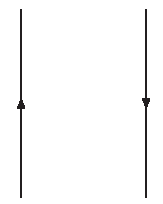
\includegraphics[scale=0.75]{holepart}
\caption{Diagrammatic representation of holes and particles, holes 
with an downward pointing arrow and particles with and upward pointing arrow.}
\label{holepart}
\end{figure}

\item The reference wavefunction $\Phi_0,$ is represented by empty
 space.

\item Dynamical operators such as the one particle and two particle
part of the Hamiltonian are depicted by horizontal dashed lines as seen in Fig.~\ref{intline}.
\begin{figure}[htp]
\centering
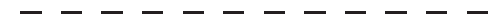
\includegraphics[scale=0.75]{interaction}
\caption{Diagrammatic representation of the interaction line.}
\label{intline}
\end{figure}

\item The cluster operators are depicted by solid horizontal lines as in Fig.~\ref{clusterline}
\begin{figure}[htp]
\centering
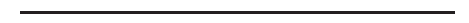
\includegraphics[scale=0.75]{cluster}
\caption{Depiction of the cluster operator.}
\label{clusterline}
\end{figure}


\item The one particle component of the Hamiltonian is represented
		by a dashed interaction line capped by an $X,$ see Fig.~\ref{hartreeX}.
\begin{figure}[htp]
\centering
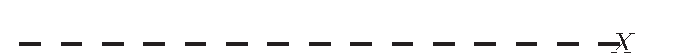
\includegraphics[scale=0.75]{hartreefockop}
\caption{Depiction of the one particle component of the Hamiltonian.}
\label{hartreeX}
\end{figure}



\item Representation of the cluster operators is seen in 
Fig.~\ref{clusterdi}. In the diagram representing the $T_1$ amplitude there
is one incoming hole line and one outgoing particle line meeting at a solid
horizontal line.


\begin{figure}[htp]
\centering
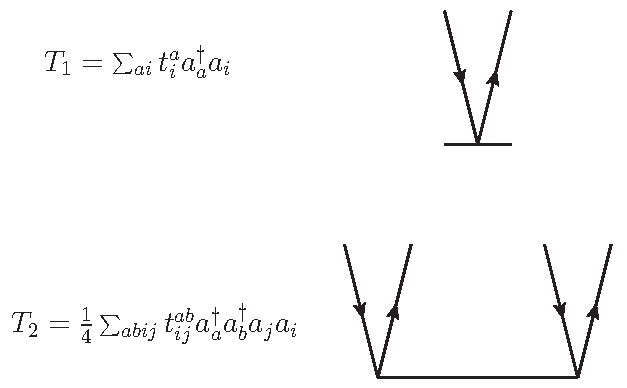
\includegraphics[scale=0.5]{clusterdi}
\caption{Diagrammatic representation of the cluster operators $T_1$
and $T_2$.}
\label{clusterdi}
\end{figure}

The diagram representing $T_2$ consists of two incoming hole lines and two
outgoing particle lines. 

\item We label  particle lines with $a,b,c,d,\cdots\,.$ and all hole lines with $i,j,k,l,\cdots\,.$.

\item We sum over internal lines, all indices associated with lines that begins and ends at operator interaction lines and do not extend to infinity above or below the diagram.

\item For each hole line, multiply with a factor of -1.

\item For each loop, multiply with a factor of -1. In Fig.~\ref{loops} we have depicted the interpretations of loops in the coupled cluster diagrams. A loop is a route a long a series of directed lines that either returns to its beginning or begins at one external line and ends at another.
\begin{figure}[htp]
\centering
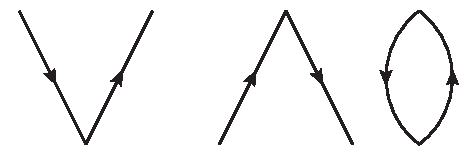
\includegraphics[scale=0.75]{loops}
\caption{Three different types of loops in the coupled cluster diagrams.}
\label{loops}
\end{figure}

\item For each pair of equivalent lines multiply with the factor $1/2$. An equivalent pair of lines are lines beginning at the same operator interaction line and ending at the same interaction line.

\item If there are $n$ equivalent vertices's in the diagram, multiply
with the factor $1/n!.$

\item For each pair of unique external hole or particle lines, multiply with
 the permutation operator $P(pq).$


\end{enumerate}
By using the above diagram rules it is possible to write diagrams
corresponding to the energy equation and amplitude equations. \\
Like the diagrams for the energy equation in Eq.~\eqref{lastformham}
\be
E=\bra{\Phi_0}H_N+H_NT_1+H_Nt_2+\frac{1}{2}H_NT^2_1+\dots \ket{\Phi_0}
\ee
can be evaluated with the above rules. The first term will not
contribute since the operator is normalized and therefore will
annihilate the vacuum state and give zero contribution.\\
\\
We will now study how the second term
\be
\bra{\Phi_0}H_NT_1\ket{\Phi_0},
\label{firstendi}
\ee
which may be depicted as a Feynman-Goldstone diagram.\\
Since we have the reference vacuum in both incoming and outgoing states there
should be no external lines, meaning that there should not be 
any line neither below or above the two horizontal operator 
lines. The $T_1$ operator stands to the right, and its 
corresponding interaction line should be in the bottom of 
the diagram. Only the one particle operator contributes since with a two 
particle operator it is impossible to draw a diagram with just internal 
lines, see Fig. \ref{firstenedi}. 
%Fig. (\ref{firstenedi}) shows the diagrammatic representation of
%the energy term $\bra{\Phi_0}H_NT_1\ket{\Phi_0}.$
%Eq. \eqref{firstendi}
\begin{figure}[htp]
\centering
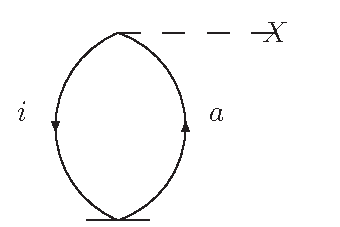
\includegraphics[scale=0.75]{firstenedi}
\caption{Diagrammatic representation of the first term in the 
ECCSD energy equation.}
\label{firstenedi}
\end{figure}
In the second contribution,
\be
\bra{\Phi_0}H_NT_2\ket{\Phi_0},
\label{secendi}
\ee
we have the reference vacuum in both incoming and outgoing state and therefore no external lines. Since the 
cluster operator is the rightmost one, the interaction line 
representing it should again be at the bottom. However, to this 
part only the two-particle operator of the Hamiltonian is 
contributing, something which should be reflected in the 
diagram. Figure \ref{secndi} shows the diagram representing Eq.~\eqref{secendi}.
\begin{figure}[htp]
\centering
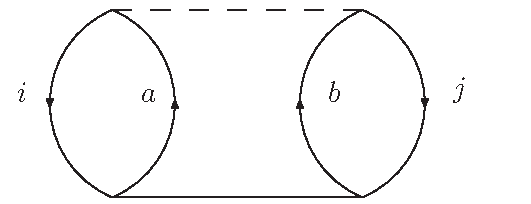
\includegraphics[scale=0.75]{secenedi}
\caption{Diagrammatic representation of the second term in the 
ECCSD energy equation.}
\label{secndi}
\end{figure}
The last part contributing to the $ECCSD$ energy equation is the
term 
\be
\frac{1}{2}\bra{\Phi_0}H_NT_1^2\ket{\Phi_0}.
\label{thirdpartendi}
\ee
The interaction lines corresponding to the two cluster operators
will again have to be drawn at the bottom of the diagram, the 
difference in this diagram, Fig.~\ref{thirdenedi}, from 
Fig.~\ref{secndi} is that the 
interaction line corresponding to the cluster operator is 
split since there are two one-excitation cluster operators to
the right in Eq.~\eqref{thirdpartendi}. 
\begin{figure}[htp]
\centering
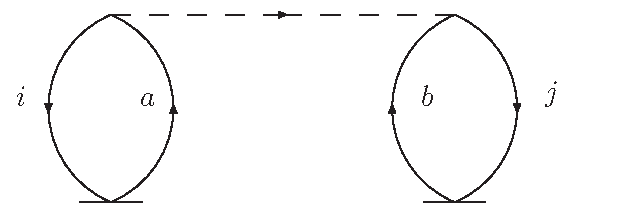
\includegraphics[scale=0.75]{thirdenedi}
\caption{Diagrammatic representation of the last term in the 
ECCSD energy equation.}
\label{thirdenedi}
\end{figure}
We can find the $T$ amplitude diagrams by using the commutators and the above diagram rules. However it is more practical to derive the amplitude equations from the amplitude diagrams. We start by
drawing all topologically distinct diagrams with  one external hole line and one external particle line for 
the $T_1$ amplitude equation. For the $T_2$ diagrams we must consider that there are two external hole 
lines and two external particle lines.\\
\\
The first leading term 
in the equation corresponding to $T_1$ consists just of the Hamiltonian, and 
only the one particle part of it contributes. Its corresponding diagram is
depicted in Fig. \ref{firstamplt1}.  
\begin{figure}[htp]
\centering
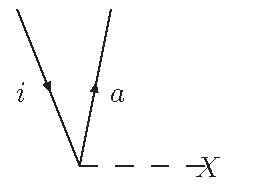
\includegraphics[scale=0.75]{firstampl}
\caption{The diagram representing the first leading term in the
$T_1$ amplitude equation.}
\label{firstamplt1}
\end{figure} 
All diagrams contributing to the $T_1$ equation can be seen in Fig.~\ref{t1_eqn_diag}.\\
\begin{figure}[htp]
%\begin{minipage}{2in}%[t]{0.5\linewidth}
\centering
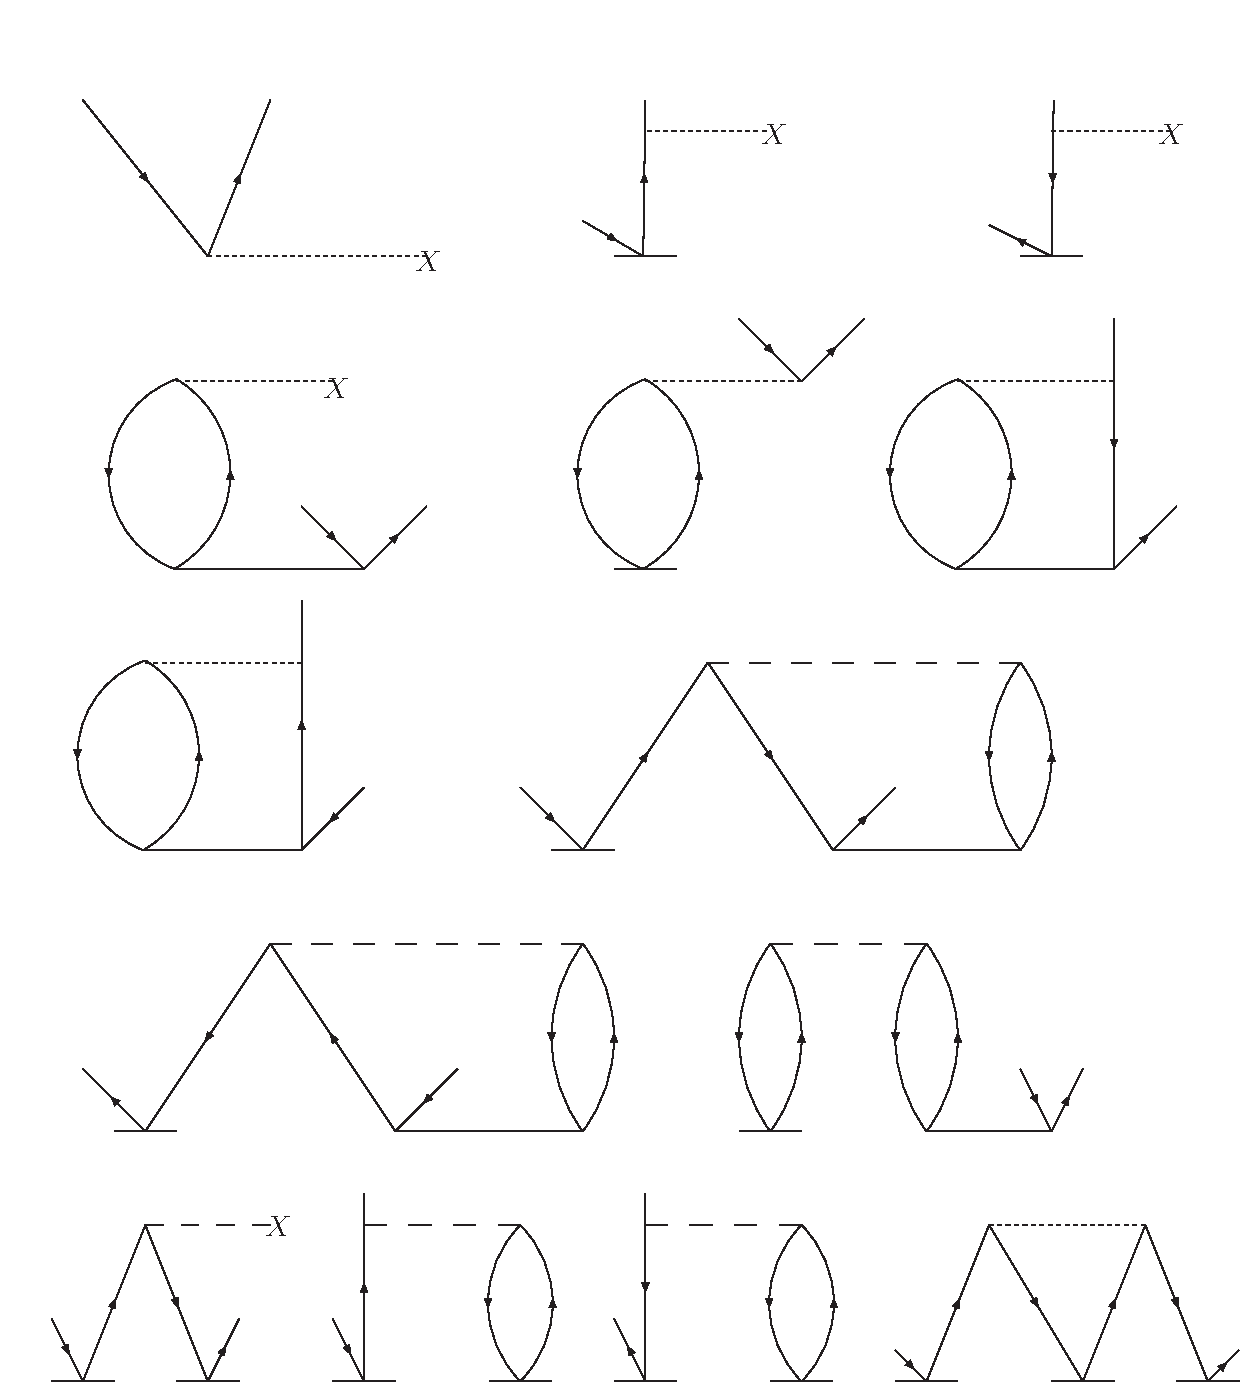
\includegraphics[scale=0.25]{t1_eqn_diag}
\caption{All diagrams contributing to the equation for solving the
$T_1$ amplitude.}
\label{t1_eqn_diag}
%\end{minipage}
\end{figure}
%\hspace{0.5cm}
%\begin{minipage}{2in}%[t]{0.5\linewidth}
In Fig.~\ref{t2_eqn_diag} we depicted all diagrams contributing to the CCD equation, while the remaining parts in a CCSD approximation are depicted in 
Fig.~\ref{t2_eqn_diag_ccsd}.  
%\end{minipage}
%\clearpage
\begin{figure}[htp]
\centering
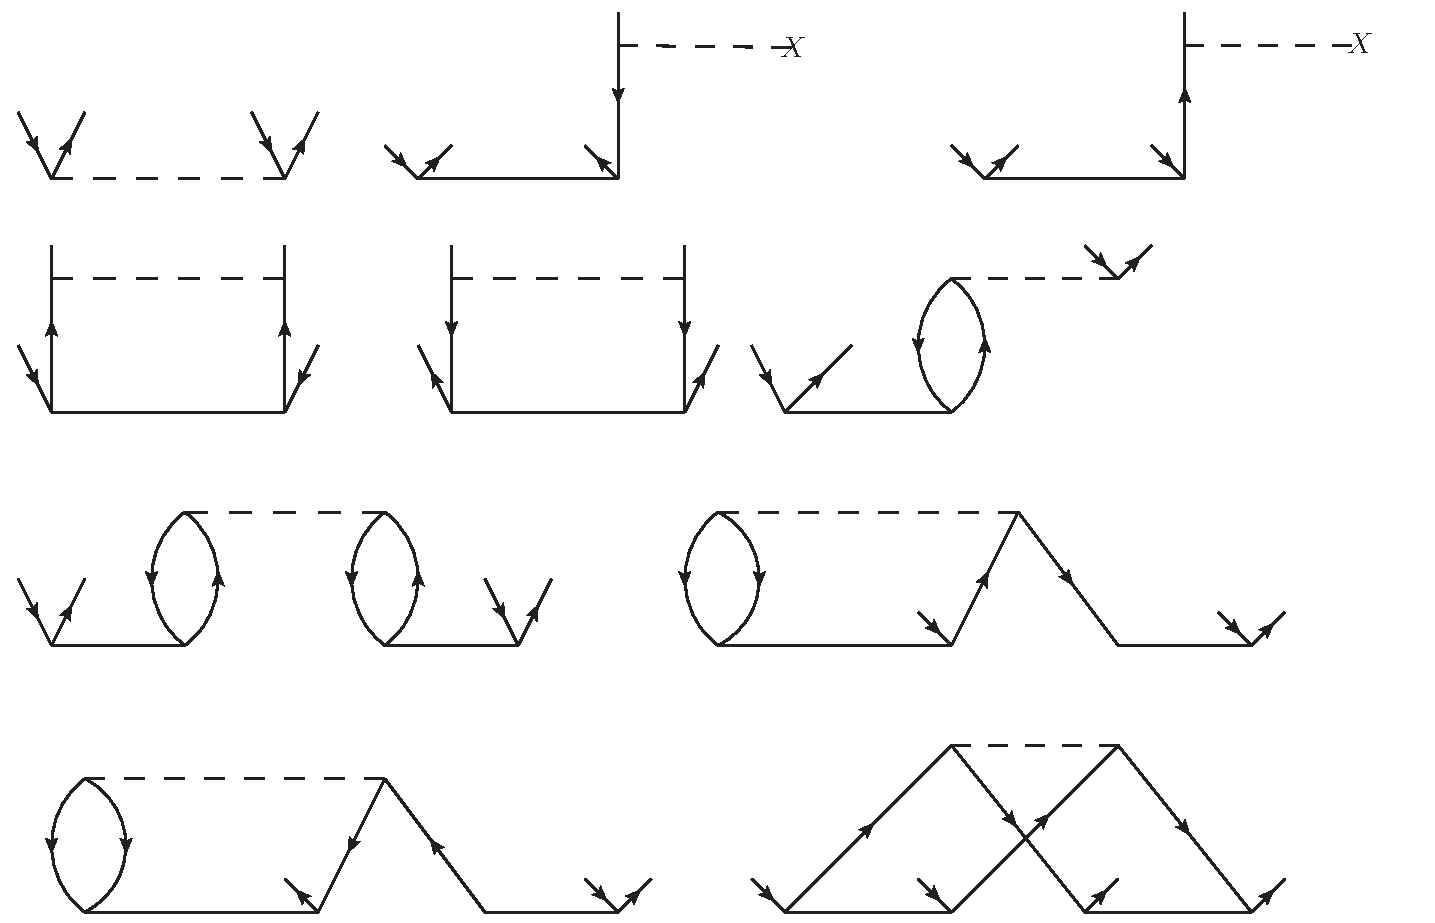
\includegraphics[scale=0.5]{t2_eqn_diag}%{CCD_diag}
\caption{All diagrams contributing to the equation for solving the
$T_2$ amplitude in the CCD approach.}
\label{t2_eqn_diag}
\end{figure}
\begin{figure}[htp]
\centering
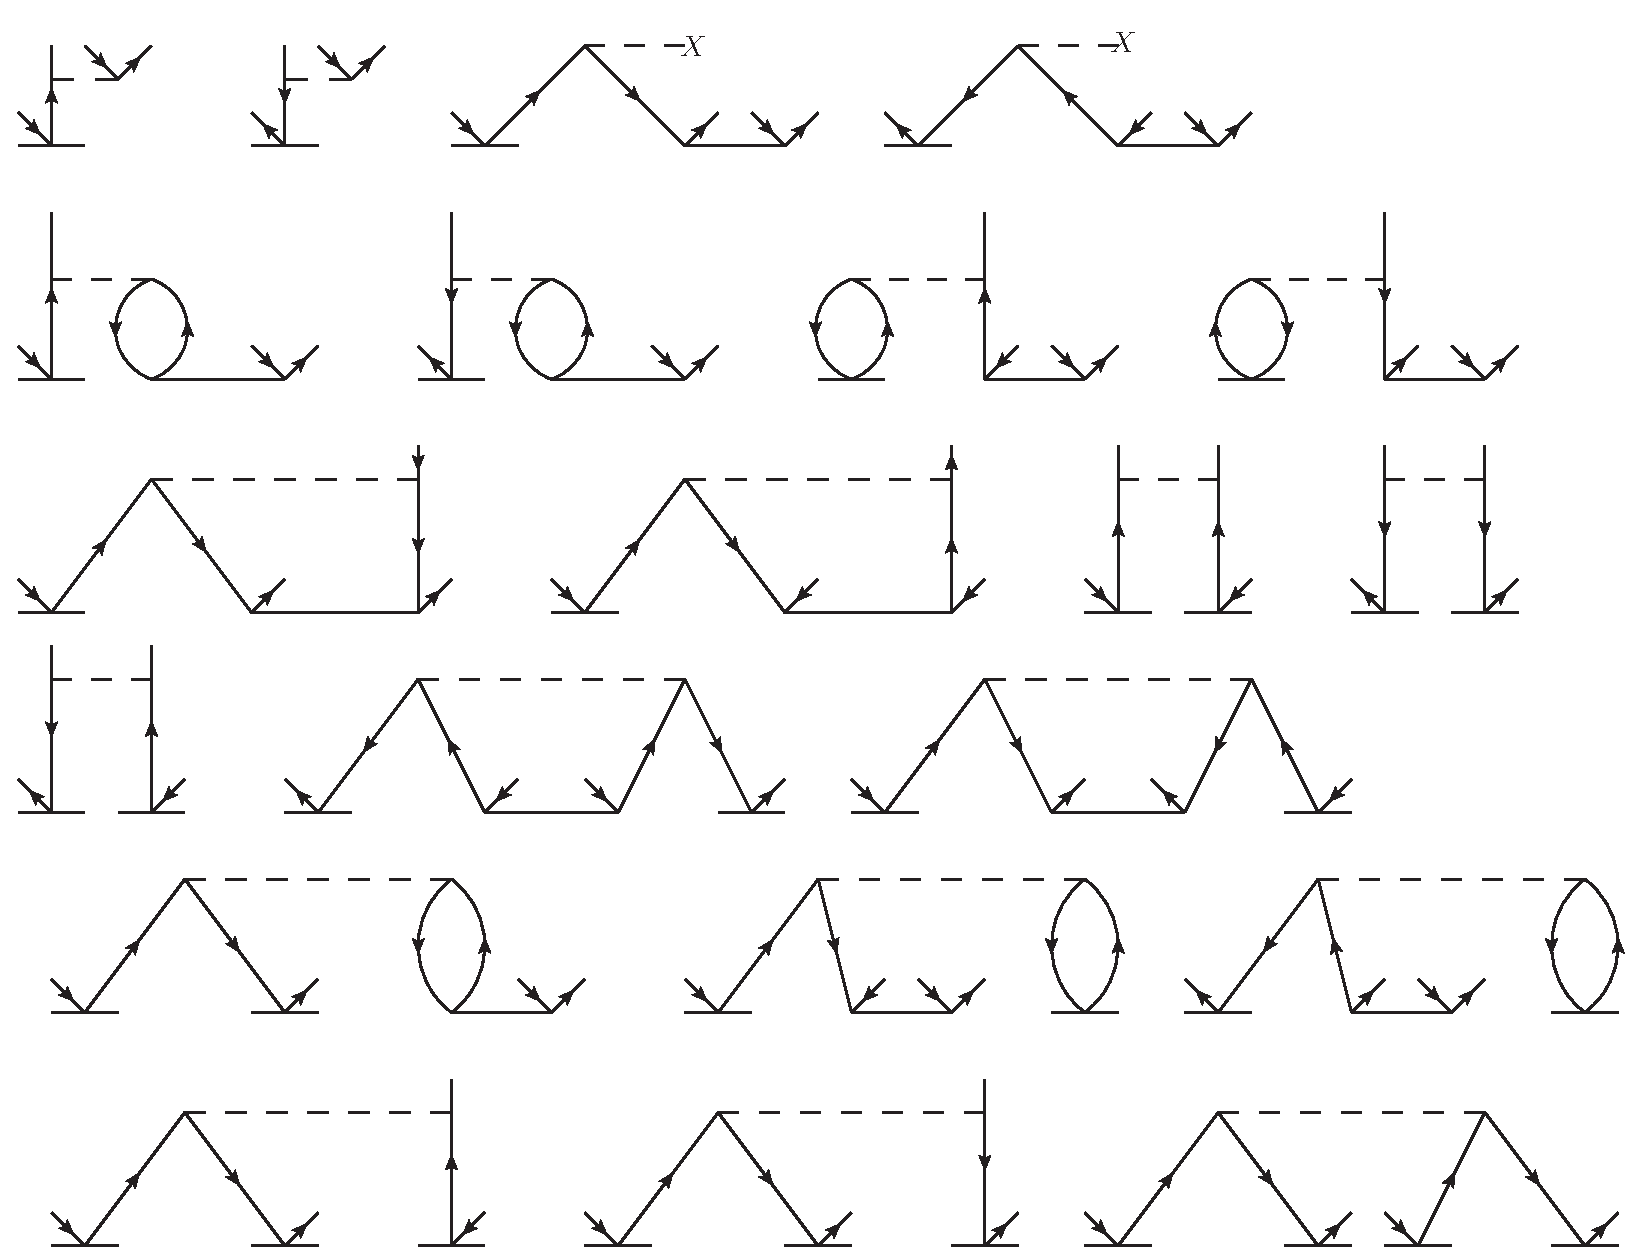
\includegraphics[scale=0.5]{t2_eqn_diag2}%{CCSD_diag}
\caption{The diagrams remaining in a CCSD approach to the
$T_2$ amplitude.}
\label{t2_eqn_diag_ccsd}
\end{figure}\\
%\clearpage
\\
To see the benefit with the diagrams, the $CCSD$ energy 
equation will now be computed from the diagrams. The total 
energy can be depicted as in Fig.~\ref{totenergydi}\\
\begin{figure}[htp]
\centering
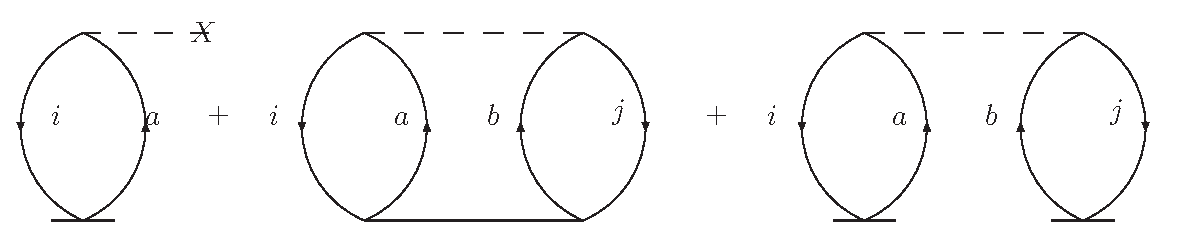
\includegraphics[width=1.0\textwidth]{energy}
\caption{The diagrams representing the total $CCSD$ 
energy.}
\label{totenergydi}
\end{figure}
The way to interpret the diagrams is from the bottom to the 
upper part. The ingoing states are 
represented by a ket vector and the outgoing by the dual bra 
vector. In the first diagram in Fig.~\ref{totenergydi} the one-excitation operator line is at the bottom. We
label each internal particle and hole line and perform a sum over all hole and particle states. We have one
hole line and one loop which together contributes as $(-1)^{1+1}=1$. On top we have a one-body
interaction line. We find that the first diagram in Fig.~\ref{totenergydi} 
should be understood as
\be
\sum_{ai}f_{ia}t^a_i,
\ee
By using the above diagram 
rules to the second diagram in Fig.~\ref{totenergydi}, we find its
matrix elements to be
\be
\frac{1}{4}\sum_{ijab}v_{ijab}t^{ab}_{ij},
\ee
where $v_{ijab}=\bra{ij}v\ket{ab}.$  We have two loops and two hole lines which together contribute with the factor $1$. We have two pairs of equivalent lines which together contribute with the factor $1/4$. A factor of $1/2$ for each pair of equivalent lines. With the same reasoning we write the last
diagram in Fig.~\ref{totenergydi} as
\be
\frac{1}{2}\sum_{ijab}\bra{ij}v_N\ket{ab}t^a_it^b_j=\frac{1}{2}\sum_{ijab}v_{ijab}t^a_it^b_j.
\ee
The factor of $1/2$ appears because of two equivalent vertices.
After summing up the energy,  the total equation becomes
\be
\sum_{ia}f_{ia}t^a_i+\frac{1}{4}\sum_{ijab}v_{ijab}t^{ab}_{ij}
+\frac{1}{2}\sum_{ijab}v_{ijab}t^a_it^b_j,
\ee
which is exactly the same as the equation got by using Wick's 
theorem.\\ 

%The same reasoning as above for the energy equation can be done
%at the $CCSD$ amplitude equations. In this case one has to take
%in consideration that the states dealed with are excited states
%projected on the normaled ordered coupled cluster Hamiltonian 
%operated on the groundstate.
%
%The leading term in the $T_1$ amplitude  equation is $\bra{\Phi^a_i}H_N\ket{\Phi_0}$. Only the one particle operator is 
%contributing here, the corresponding diagram would be 
%
%\begin{figure}[htp]
%\centering
%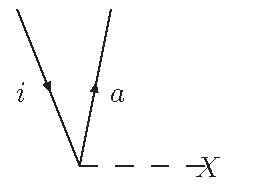
\includegraphics{firstampl}
%\caption{The diagram representing the first leading term in the
%$T_1$ amplitude equation. The interpretation is $f_{ai}$ }
%\label{firstamplt}
%\end{figure}
%
%Converting the diagram in Fig. (\ref{firstamplt}) to an equation
%would give the result $f_{ai}.$
%
%The first leading term in the $T_2$ amplitude equation is
%$\bra{\Phi^{ab}_{ij}}H_N\ket{\Phi_0},$ only the two-particle 
%operator is contributing to this part and the diagram is as is 
%shown in Fig. (\ref{secamplt})
%
%\begin{figure}[htp]
%\centering
%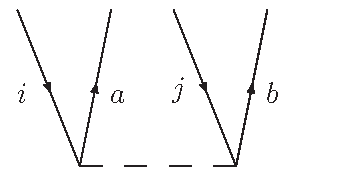
\includegraphics{secampl}
%\caption{The diagram representing the first leading term in the
%$T_2$ amplitude equation. It is representing the equation 
%$V_{ijab}$ }
%\label{secamplt}
%\end{figure}
%
%The matrix element, Fig(\ref{secamplt}), is $\bra{ab}V\ket{ij}.$
%\clearpage
\section{Computation of the equations}
\label{compofccsd}

This section will treat the computational approach for solving the amplitude
equations as Eqs.~\eqref{firstamplitude} and \eqref{secondamplitude}.
It is not always clear how one should approach the equations. 
A first approach could be to rearrange the equations to provide a more handy form. As an example the first few terms of Eq. \eqref{firstamplitude}, could be written as
\be
0=f_{ai}+f_{aa}t^a_i-f_{ii}t^a_i+\sum_c(1-\delta_{ca})f_{ac}t^c_i-\sum_k (1-\delta_{ik})f_{ik}t^a_k+\cdots
\label{firstfirstampl}
\ee
By defining 
\be
D^a_i=f_{ii}-f_{aa}
\ee
we rewrite Eq.~\eqref{firstfirstampl} as 
\be
D^a_it^a_i=f_{ai}+\sum_c(1-\delta_{ca})f_{ac}t^c_i-\sum_k(1-\delta_{ik})f_{ik}t^a_k+\cdots.
\ee
By also defining 
\be
D^{ab}_{ij}=f_{ii}+f_{jj}-f_{aa}-f_{bb}
\ee
the $T_2$ amplitude can be rewritten as
\be
D^{ab}_{ij}t^{ab}_{ij}=\bra{ab}v\ket{ij}+P(ab)\sum_c(1-\delta_{bc})f_{bc}t^{ac}_{ij}-P(ij)\sum_{k}(1-\delta_{kj})f_{kj}t^{ab}_{ik}+\cdots
\ee
The equations above have to be solved iteratively. A starting point for $t^a_i$ and $t^{ab}_{ij}$ may be obtained by setting all of the amplitudes on the right-hand side to zero. The initial guess for the amplitudes are then
\be
t^a_i=f_{ai}/D^a_i,
\ee 
for the $T_1$ amplitude and 
\be
t^{ab}_{ij}=\bra{ab}v\ket{ij}/D^{ab}_{ij}
\ee
for the $T_2$ amplitude.\\
These initial guesses have to be inserted on the right-hand side of the 
equations and then subsequently used to obtain new 
amplitudes. This process is continued until an explicit convergence is 
reached.\\
\\
In momentum space and a plane wave basis in addition to the sum over single-particle states in the energy and amplitude equations, we will
also have to integrate over the momentum for each single-particle state. Holes have momentum less than the 
Fermi momentum $k_f$, while particles have momentum greater than $k_f$.\\
\\
The single-particle functions $\varphi$ are defined as plane-waves
\beq
\varphi=\frac{1}{\sqrt{\Omega}}e^{i\bold k\bold r},
\eeq
where the volume, $\Omega$ is infinite, $k$ denotes the principal wave-number and $r$ the radial coordinate.
When we calculate interactions it is convenient to do a so-called partial wave-expansion.
We expand the exponential as a sum of Legendre polynomials and spherical Bessel functions
\beq
e^{ikr}=\sum_{l=0}^\infty(2l+1)i^lj_l(kr)P_l(\Omega_{k,r}),
\eeq
where the spherical Bessel functions $j_l(kr)$ depends on the radial part of the momentum and position vector, see appendix \ref{app:leg} and \ref{app:bess} for details about the functions. The Legendre polynomials $P_l$ depends on 
$\Omega_{k,r}=\bold k\cdot \bold r/(|k||r|)$, which is the cosine angle between $\bold k$ and $\bold r$. The sum goes over orbital momentum $l$.\\ 
\\
We saw in Eqs.~\eqref{firstamplitude} and \eqref{secondamplitude} that there
are many diagrams contributing to the amplitude equations, as many diagrams
as terms in the equations. It requires a lot of time computing all these
diagrams separately, therefore it is wise to 
factorize the diagrams. This can be done, since the coupled cluster diagrams do not have any denominators in their's expressions,
in contrast to the diagrams in perturbation theory. 
Instead of computing the same factors several times, we compute it once and
multiply it with the corresponding terms, as explained by Ref.~\cite{bartlett:291}. In this work the factorization used is the same as the one used by Ref.~\cite{hagen:034302}.

\section{Further analysis of the coupled cluster method} In the section on
perturbation theory we derived the diagram rules and draw diagrams
up to third order.  In section \ref{compofccsd} we showed how to solve the CCSD equations. With an initial guess for the $T_2$ amplitude as
\be\frac{\bra{ab}v\ket{ij}}{f_{ij}-f_{ab}}\ee 
and insert it in the CCSD energy equation gives us
\be
E_{T_2}= \frac{1}{4}\sum_{\substack{i,j \\a,b}} v_{ijab}t^{ab}_{ij}=\frac{1}{4}\sum_{\substack{i,j \\a,b}}\frac{\bra{ij}v\ket{ab}\bra{ab}v\ket{ij}}{f_{ij}-f_{ab}},
\ee
which is exactly the same expression as the second order contribution to the energy in perturbation theory. 
By doing more of the iterations, the coupled cluster method will also include diagrams from third and fourth
order in perturbation theory.\\ % We see that
%there is a fine connection between the coupled cluster calculations and calculations with perturbation theory.\\
\\
A convenient property of the coupled cluster method is that it is size
consistent and size extensive. By size consistent we mean that computing the
energy of two nuclei with an infinite distance between them is just to compute
the two energies separately. As an example we consider two
nuclei, $A$ and $B.$
\be
\begin{split}
&\ket{\Phi_0} = \ket{\Phi^A_0}\ket{\Phi^B_0}\\
&e^T\ket{\Phi_0}=e^{T_A+T_B}\ket{\Phi^A_0}\ket{\Phi^B_0}=e^{T_A}\ket{\Phi^A_0}e^{T_B}\ket{\Phi^B_0}.\\
\end{split}
\ee
With the Hamiltonian on the form $H=H_A + H_B$ the energy of the combined system  sums up to  
\be
E_{CC}= E^A_{CC} + E^B_{CC}.
\ee
With size extensive means that the energy is linearly dependent on the number of particles present. 




















